%************************************************
\chapter{Introduction to Learning-to-Rank}
Different definitions of Learning-to-Rank exist. In general, all ranking methods that use machine learning technologies to solve the problem of ranking are called Learning-to-Rank methods. Figure \ref{fig:discriminative_training} describes the general process of machine learning. It shows training elements from an input space that are mapped to an output space using a model such that the difference between the actual labels of the training elements and the labels predicted with with the model are minimal in terms of a loss function.
\begin{figure}[!h]
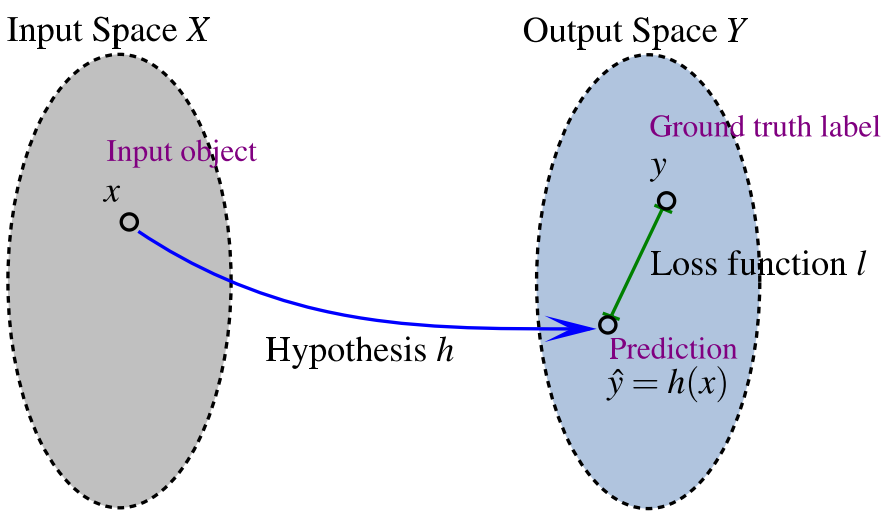
\includegraphics[scale=0.26]{gfx/descriminative_training}
\caption{Machine learning framework for Learning-to-Rank, obtained from Liu\cite{Liu2007}}
\label{fig:discriminative_training}
\end{figure}\\
Liu \cite{Liu2007} proposes a more narrow definition and only considers ranking methods to be a Learning-to-Rank method when it is \emph{feature based} and uses \emph{discriminative training}, which are itself defined as follows:
\begin{description}
\item[Feature Based]{\emph{Feature based} means that all documents under investigation are represented by feature vectors that reflect the relevance of the documents to the query.}
\item[Discriminative Training]{\emph{Discriminative training} means that the learning process can be well described by the four components of discriminative learning. That is, a Learning-to-Rank method has its own \emph{input space}, \emph{output space}, \emph{hypothesis space}, and \emph{loss function}, like the machine learning process described by Figure \ref{fig:discriminative_training}. \emph{Input space}, \emph{output space}, \emph{hypothesis space}, and \emph{loss function} are hereby defined as follows:
	\begin{description}
	\item[Input Space]{contains the objects under investigation. Usually objects are represented by feature vectors, extracted according to different applications.}
	\item[Output Space]{contains the learning target with respect to the input objects.}
	\item[Hypothesis Space]{defines the class of functions mapping the input space to the output space. The functions operate on the feature vectors of the input object, and make predictions according to the format of the output space.}
	\item[Loss Function]{in order to learn the optimal hypothesis, a training set is usually used, which contains a number of objects and their ground truth labels, sampled from the product of the input and output spaces.}
	\end{description}
	}
\end{description}


Figure \ref{fig:ltr_framework} shows how the machine learning process as described in Figure \ref{fig:discriminative_training} typically takes place in a ranking scenario. A set of queries $q_i$ with $n > i > 1$, the documents associated with these queries which are represented by feature vector $x_i$, and the relevant judgments of those documents $y_i$ are used together to train a model $h$, that can predict a ranking of the documents $y_i$, such the difference between the document rankings predicted by $h$ and the actual optimal rankings based on $y_i$ is are minimal in terms of a loss function.
\begin{figure}[!h]
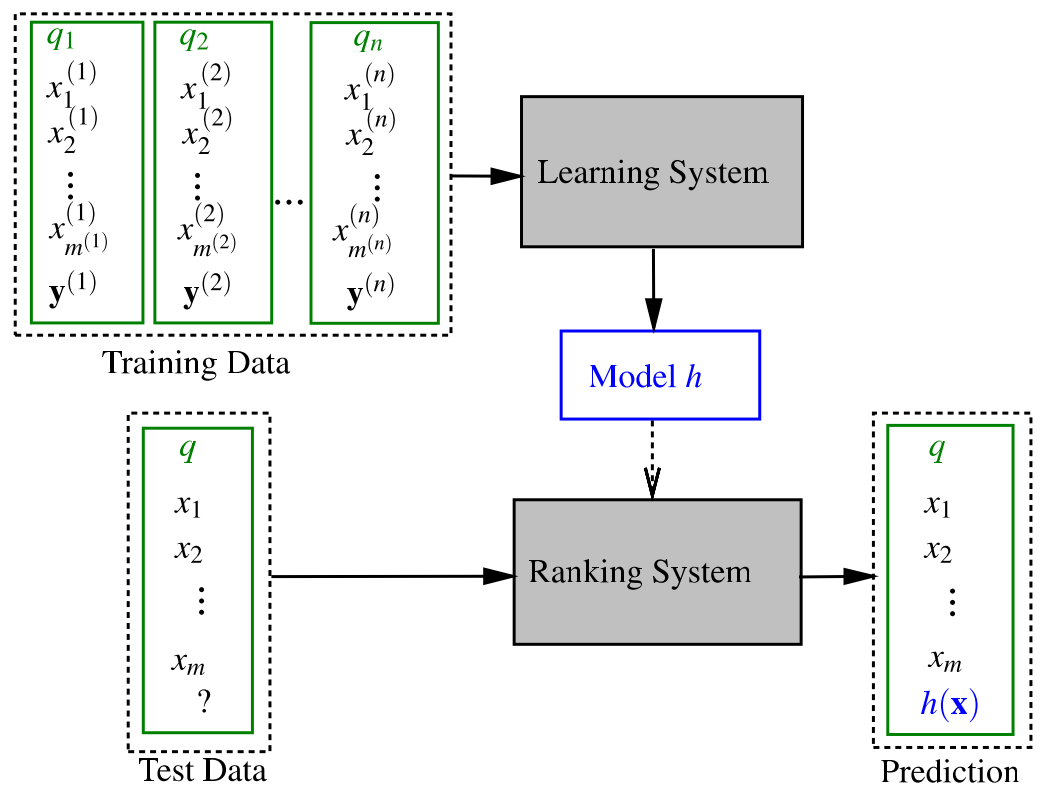
\includegraphics[scale=0.25]{gfx/ltr_framework}
\caption{A typical Learning-to-Rank setting, obtained from Liu\cite{Liu2007}}
\label{fig:ltr_framework}
\end{figure}\\

The predictions and the loss function might either be defined for:
\begin{enumerate}
\item the relevance of a single document
\item the classification of the most relevant document out of a document-pair
\item the ranking of documents directly
\end{enumerate}
These three approaches are in literature respectively called the pointwise approach, the pairwise approach and the listwise approach. In the following sections we will further describe the three different approaches in Learning-to-Rank.

\section{Pointwise Approach}

\section{Pairwise Approach}
\section{Listwise Approach}
\section{Evaluation Methods}
\subsection{Normalized Discounted Cumulative Gain}
\subsubsection{Cumulative Gain}
\subsubsection{Discounted Cumulative Gain}
\ac{DCG}
\subsubsection{Normalized Discounted Cumulative Gain}
\ac{nDCG}
\subsection{Expected Reciprocal Rank}
\ac{ERR}